\documentclass{eic-bcc-tcc}

%-----------------------------------------------
% Metadados do Trabalho
%-----------------------------------------------
\title{Título do Trabalho de Conclusão de Curso sem Abreviações: Subtítulo se Houver}
\titleen{Title of the Final Course Work without Abbreviations: Subtitle if Any}


% Nome completo do/da(s) autor(es)
% \addstudent[Full Name]{Nome Completo}
% O comando recebe um parâmetro opcional para a formatação dos nomes em inglÊs
\addstudent[First Full Name]{Primeiro Nome Completo}
\addstudent[Second Full Name]{Segundo Nome Completo}
\addstudent[Third Full Name]{Terceiro Nome Completo}


% Nomes do/a(s) orientador/a(s) e participantes da banca. Nos exemplos abaixo, utiliza-se após o nome a titulação correspondente. Caso a titulação não seja D.Sc., utilizar a adequada (p.ex., Dr. Ing., M.Sc., Esp., entre outras)
% Os comandos \advisor e \coadvisor possuem um parâmetro opcional m/f para alterar o texto para orientador ou orientadora
\advisor[f]{Nome do(a) Orientador(a), D.Sc.\footnotemark[1]} 
\coadvisor{Nome do(a) Coorientador(a), D.Sc.\footnotemark[1]}


% Membros da Banca para folha de aprovação
\addboardmember{Membro Interno}{Nome Membro Interno, D.Sc.\footnotemark[1]}
\addboardmember{Membro Externo}{Nome Membro Externo, D.Sc.\footnotemark[1] \footnotetext[1]{Caso a titulação não seja D.Sc., utilizar a adequada (p.ex., Dr. Ing., M.Sc., Esp., entre outras)}}

% Ano da defesa
\date{2025}


%-----------------------------------------------
% Abreviações
%-----------------------------------------------
% \newacronym{label}{sigla}{descrição} - Define um novo acrônimo
\newacronym{cefet}{Cefet/RJ}{Centro Federal de Educação Tecnológica Celso Suckow da Fonseca}
\newacronym{tcc}{TCC}{Trabalho de Conlusão de Curso}
\newacronym{abnt}{ABNT}{Associação Brasileira de Normas Técnicas}
\newacronym{ia}{IA}{Inteligência Artificial}


\begin{document}

%-----------------------------------------------
% Elementos pré-textuais
%-----------------------------------------------
\maketitle

\begin{dedicatoria}
A dedicatória é composta de um texto curto onde o autor dedica o trabalho a alguém, como forma de homenagem ou reverência. Esse é um elemento facultativo do TCC.
\end{dedicatoria}


\begin{agradecimentos}
Os agradecimentos contêm a relação de pessoas que contribuíram para o sucesso do TCC.
Trata-se, então, de espaço para identificar e reconhecer essa contribuição, na forma de agradecimento e homenagem.

Esse é um elemento facultativo do TCC; porém, se houver algum apoio financeiro para o desenvolvimento do projeto, como bolsa de iniciação científica ou bolsa de financiamento do projeto, o agradecimento passa a ser obrigatório, devendo-se, minimamente, agradecer ao apoio financeiro obtido.
\end{agradecimentos}


% Cria a folha de aprovação. Adicione um arquivo termo.pdf com as assinaturas da baca para substituir o termo gerado.
\makeapproval


\begin{resumo}
Elemento obrigatório, constituído de uma sequência de frases concisas e objetivas, fornecendo uma visão rápida e clara do conteúdo do estudo. O texto deverá conter no máximo 500 palavras e ser antecedido pela referência do estudo, além de não conter citações. O resumo deve ser redigido em parágrafo único.
Um bom resumo apresenta os itens 
\textbf{Contextualização:} descreve o contexto do trabalho sendo apresentado; 
\textbf{Gap:} apresenta o que não está coberto pela literatura; 
\textbf{Objetivo:} indicando o propósito do trabalho; 
\textbf{Metodologia:} como o trabalho pretende alcançar o objetivo; e 
\textbf{Resultados:} resumo dos principais resultados para estimular a leitura do trabalho, seguido das principais conclusões.
Abaixo do resumo, apresentamos as palavras-chave que identificam o trabalho, permitindo uma classificação de indexação para facilitar sua localização por mecanismos de pesquisa apropriados. Utilizamos como palavras-chave as mais representativas do conteúdo do trabalho. Deve-se designar de três a cinco palavras-chaves, separadas entre si por ponto e finalizadas também por ponto.

\palavraschave{Palavra-chave 1. Palavra-chave 2. Palavra-chave 3. Palavra-chave 4. Palavra-chave 5.}
\end{resumo}


\begin{abstract}
Mandatory element, consting of a sequence of concise and objective sentences, providing a quick and clear overview of the study's content. The text must contain a maximum of 500 words and be preceded by the study's reference. It should not include citations and must be written as a single paragraph.
A good abstract presents the following elements:
\textbf{Contextualization:} describes the context of the study being presented;
\textbf{Gap:} indicates what is not yet covered in the literature;
\textbf{Objective:} states the purpose of the study; 
\textbf{Methodology:} explains how the study intends to achieve its objective; and
\textbf{Results:} summarizes the main findings to encourage reading of the full work, followed by the main conclusions.
Below the abstract, keywords are provided to identify the study, allowing for indexing classification and facilitating its retrieval through appropriate search mechanisms. The most representative words related to the content of the work should be used. Three to five keywords must be provided, separated by periods and ending with a period as well.

\keywords{Keyword 1. Keyword 2. Keyword 3. Keyword 4. Keyword 5.}
\end{abstract}

% Lista de Figuras
\listoffigurespage

% Lista de Tabelas
\listoftablespage

% Lista de acrônimos
\listofacronymspage

% Sumário
\tableofcontentspage

% --- ELEMENTOS TEXTUAIS ---
\mainmatter


\chapter{Escrita de um TCC}

\section{Forma de Escrita}

A forma de escrita varia de acordo com o estilo do(s) orientador(es) e do(s) discente(s), mas existem alguns aspectos que devem ser atentados. Em textos científicos, as frases devem ser curtas, para não gerar ambiguidade. Pode-se dizer, genericamente, que um parágrafo é constituído por pelo menos três frases. Adicionalmente, cada parágrafo tem uma única ideia central, \textit{i.e.}, uma frase curta que sumariza o parágrafo.

O texto de um TCC como um todo precisa estar coeso. Para tanto, é necessário que haja o encadeamento dos seus parágrafos. A conexão dos parágrafos é feita a partir da concatenação de suas ideias centrais. Desta forma, a ideia central de cada parágrafo leva à ideia central do próximo e assim por diante.

Para facilitar o entendimento, tente analisar as ideias centrais dos dois primeiros parágrafos desta seção. A do primeiro pode ser entendida como ``Cada parágrafo tem uma ideia central e contém, no mínimo, três frases curtas''. A ideia central do segundo parágrafo diz que ``O encadeamento de um TCC é feito a partir do encadeamento de suas ideias centrais''. Observe que a ideia central do primeiro conduz à ideia central do segundo, estabelecendo uma relação de dependência. Este tipo de organização deve estar presente ao longo do texto todo.

\section{Estrutura Básica de um TCC}

Um \gls{tcc} é constituído pelos artefatos computacionais produzidos, e principalmente por este documento (monografia). A estrutura básica deste documento é flexível, mas deve conter, no mínimo, os seguintes capítulos: 1 – Introdução, 2 - Fundamentação Teórica\footnote{O nome da seção pode ser alterado para ficar mais condizente com o trabalho}, 3 - Desenvolvimento\footnote{O nome da seção pode ser alterado para o nome principal do artefato}, 4 - Avaliação Experimental, 5 – Conclusão (ou Considerações Finais), e Referências.

Estes itens são mais bem descritos em cada capítulo, mas em linhas gerais, a Introdução (Capítulo~\ref{cha:introducao}) é constituída pela motivação, definição do problema, objetivos e organização do trabalho. Já a fundamentação teórica (Capítulo~\ref{cha:fundamentacao}) consiste em apresentar os principais conceitos. Os trabalhos relacionados (Capítulo~\ref{cha:relacionados}) apresenta os principais trabalhos relacionados, por meio de um mapa sistemático, que compreendem o domínio do problema envolvido na solução. O desenvolvimento (Capítulo~\ref{cha:desenvolvimento}) contempla a modelagem do domínio do problema, modelo teórico e aspectos relacionados ao desenvolvimento da solução. A avaliação experimental (Capítulo~\ref{cha:avaliacao}) compreende uma avaliação qualitativa e/ou quantitativa do trabalho. Finalmente, a conclusão (Capítulo~\ref{cha:conclusao}) apresenta uma sumarização dos principais resultados do trabalho, limitações e trabalhos futuros.

Cada capítulo pode ser subdividido em seções. Os comandos \texttt{section}, \texttt{subsection}, \texttt{subsubsection} e \texttt{paragraph} criam essa estrutura conforme necessário. Abaixo são apresentados exemplos dos comandos. Repare como essas seções são apresentadas no sumário.

\section{O TÍTULO DE UMA SEÇÃO SECUNDÁRIA} % Deve estar todo em maiúsculo
\label{sec:nome} % permite a referência para essa seção
Texto da seção secundária

\subsection{O Título de uma Seção Terciária} % Deve estar com a primeira letra das palavras em maiúsculo
\label{sub:nome} % permite a referência para essa seção
Texto da seção terciária

\subsubsection{O título de uma seção quaternária} % Deve estar com apenas a primeira letra em maiúsculo
\label{ssub:nome} % permite a referência para essa seção
Texto da seção quaternária

\paragraph{O título de uma seção quinária} % Deve estar com apenas a primeira letra em maiúsculo
\label{par:nome} % permite a referência para essa seção
Texto da seção quinária


\section{Elementos pré-textuais}
Os elementos pré-textuais definem as informações iniciais do texto, como capa, contra-capa, ficha catalográfica, dedicatória, agradecimentos, termo de aprovação, resumo, \textit{abstract}, as listas de figuras, tabelas, acrônimos e sumário.

\subsection{Lista de Figuras}

Lista as figuras apresentadas ao longo do \gls{tcc}. Para incluir uma figura, utiliza-se o ambiente \verb|figure|, cujo resultado é apresentado na Figura~\ref{fig:exemplo}.

\begin{figure}[h]
    \centering
    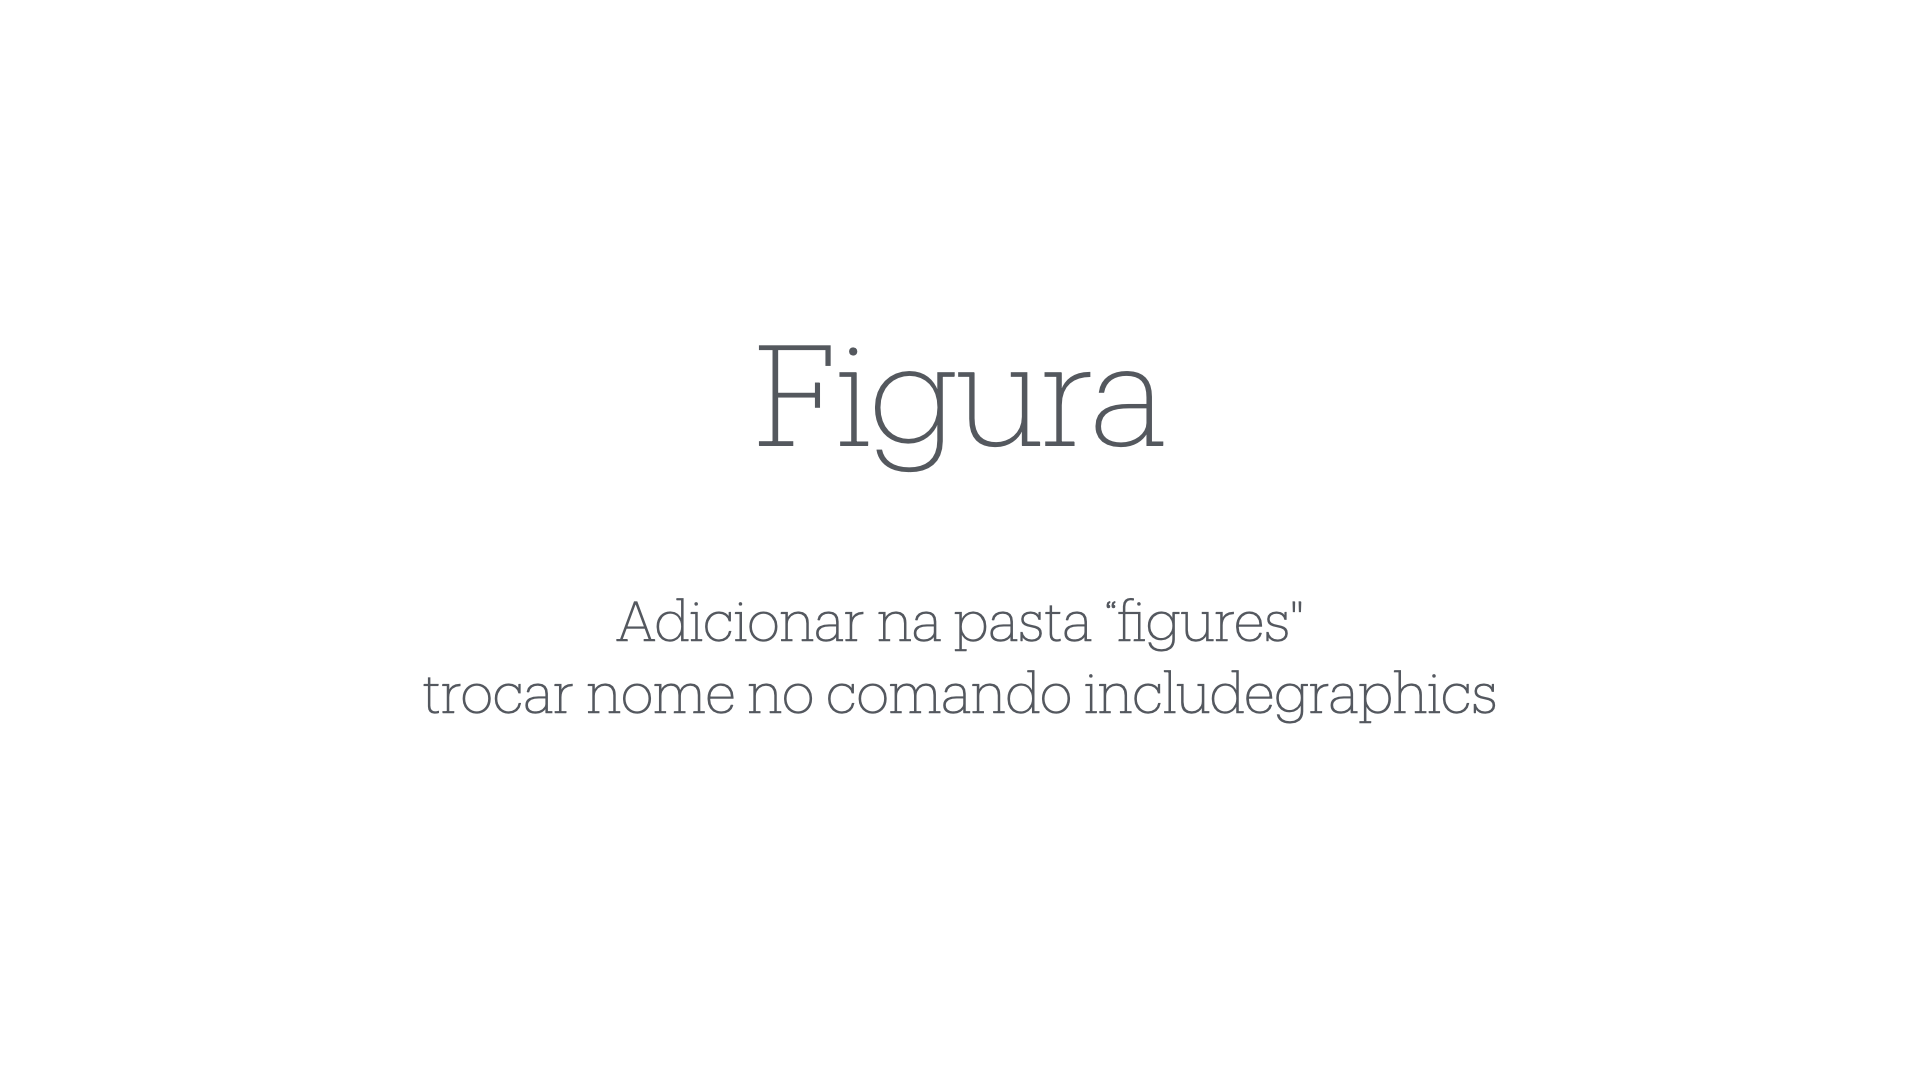
\includegraphics[width=0.6\textwidth]{figuras/figure.png}
    \caption{Exemplo de figura}
    \label{fig:exemplo}
\end{figure}

A Figura~\ref{fig:exemplo} é gerada pelo comando a seguir:

\begin{verbatim}
\begin{figure}[h]
    \centering
    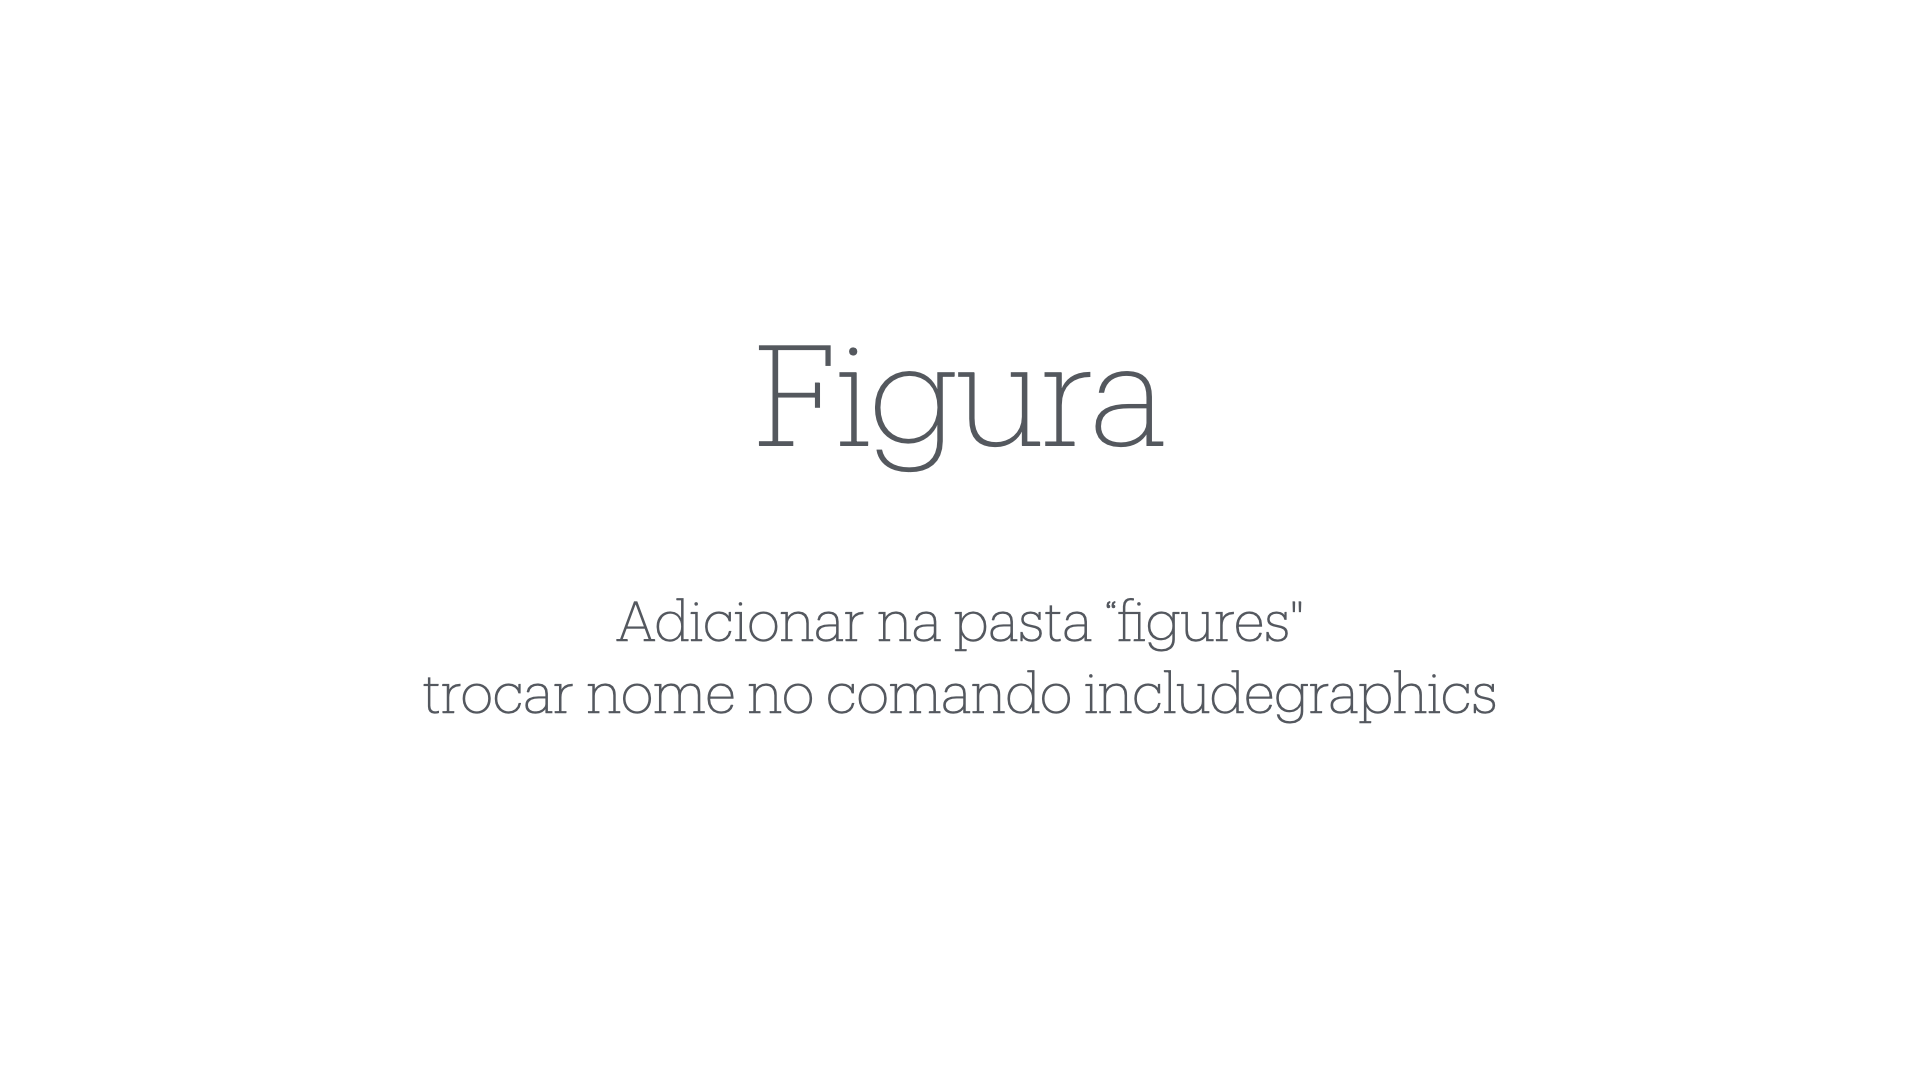
\includegraphics[width=0.7\textwidth]{figuras/figure.png}
    \caption{Exemplo de figura}
    \label{fig:exemplo}
\end{figure}
\end{verbatim}

Para mais informações sobre como incluir figuras no TCC, recomenda-se a leitura da referência \url{https://en.wikibooks.org/wiki/LaTeX/Floats,_Figures_and_Captions}.


\subsection{Lista de Tabelas}

Lista as tabelas apresentadas ao longo do \gls{tcc}. Para incluir uma tabela, utiliza-se o ambiente \verb|table|, conforme o exemplo abaixo.

\begin{verbatim}
\begin{table}[h]
    \centering
    \caption{Exemplo de Tabela}
    \label{tab:exemplo}
    \begin{tabular}{c|c}
        \hline
        \textbf{Coluna 1} & \textbf{Coluna 2} \\
        \hline
        célula 1 & célula 2 \\
        célula 3 & célula 4 \\
        \hline
    \end{tabular}
\end{table}
\end{verbatim}

O resultado do comando acima é apresentado na Tabela~\ref{tab:exemplo}.

\begin{table}[h]
    \centering
    \caption{Exemplo de Tabela}
    \label{tab:exemplo}
    \begin{tabular}{c|c}
        \hline
        \textbf{Coluna 1} & \textbf{Coluna 2} \\
        \hline
        célula 1 & célula 2 \\
        célula 3 & célula 4 \\
        \hline
    \end{tabular}
\end{table}

Para mais informações sobre como incluir tabelas no TCC, recomenda-se a leitura da página \url{https://en.wikibooks.org/wiki/LaTeX/Floats,_Figures_and_Captions}


\subsection{Lista de Acrônimos}

A lista de acrônimos organiza uma relação das abreviaturas e siglas com os seus respectivos significados, por ordem alfabética (exemplo: \textbf{TCC} Trabalho de Conclusão de Curso). No texto do trabalho, o acrônimo deve estar entre parênteses, logo após a primeira apresentação de seu significado. Nas próximas ocorrências de texto que mencionam o significado do acrônimo, tiramos o significado e usamos apenas o acrônimo, conforme abaixo:
\begin{itemize}
    \item apresentação do acrônimo em sua primeira utilização do texto: ``... \acrfull{tcc} ...'';
    \item utilização do acrônimo no restante do texto: ``... um \acrshort{tcc} deve ...''.
\end{itemize}

Os comandos \texttt{gls}, \texttt{glspl}, \texttt{acrshort}, \texttt{acrlong} e \texttt{acrfull} podem ser utilizados para controlar a apresentação de acrônimos. O comando \verb|\gls{label}| usa o acrônimo de forma inteligente, abrindo apenas a primeira utilização no texto. O comando \verb|\glspl{label}| funciona igual ao comando anterior, mas apresenta a forma no plural. Por exemplo, \verb|\glspl{tcc}| apresenta \glspl{tcc}. O comando \verb|\acrshort{label}| força a apresentação da forma abreviada. Por exemplo, \verb|\acrshort{tcc}| apresenta \acrshort{tcc}. O comando \verb|\acrlong{label}| obriga a apresentação da forma extensa. Por exemplo, \verb|\acrlong{tcc}| apresenta \acrlong{tcc}. O comando \verb|\acrfull{label}| direciona a apresentação da forma completa. Por exemplo, \verb|\acrfull{tcc}| apresenta \acrfull{tcc}.


\section{Referências}

As referências devem conter a identificação dos trabalhos e pesquisas citados (referenciados) ao longo do trabalho, conforme as normas de formatação definidas pela \gls{abnt}.

O uso de referências ao longo do texto é feito utilizando o comando \verb|\cite{key}|. A chave utilizada para citação deve estar cadastrada no arquivo \texttt{referencias.bib} para correto funcionamento. Sendo assim, o comando \verb|\cite{livro}| cita a referência de um livro produzindo \cite{livro}, enquanto o comando \verb|\cite{artigo}| cita a referência de um artigo produzindo \cite{artigo}.

É possível citar mais de uma referência de uma só vez. Assim, \verb|\cite{livro,artigo}| produz \cite{livro,artigo}. Já o comando \verb|\citeonline{artigo}| produz \citeonline{artigo} para referências diretas.

As informações das referências devem ser cadastradas no arquivo \texttt{referencias.bib}. Como exemplo, o arquivo traz uma referência para um artigo e para um livro, conforme o exemplo abaixo:
\begin{verbatim}
@book{livro,
    author = {Autor, A. and Autor, B.},
    title = {Título do Livro},
    publisher = {Editora},
    year = {2023},
    address = {Cidade}
}

@article{artigo,
    author = {Autor, C. and Autor, D.},
    title = {Título do Artigo},
    journal = {Nome do Periódico},
    volume = {10},
    number = {2},
    pages = {100-120},
    year = {2024}
}
\end{verbatim}

Para informações adicionais sobre como cadastrar outros tipos de referências, recomenda-se a leitura complementar \url{https://en.wikibooks.org/wiki/LaTeX/Bibliography_Management#Standard_templates}.


\section{Apêndices}

Os apêndices compõem os elementos pós-textuais do \gls{tcc} e são formados por todos os materiais complementares que possibilitem uma melhor compreensão do \gls{tcc}. Podemos colocar como apêndices o manual de usuário, as listagens de programas e as estatísticas do estudo realizado, dentre outros conteúdos.

\section{Anexos}

Os anexos, assim como os apêndices. são elementos pós-textuais do \gls{tcc} que conspiram de forma complementar na enriquecimento da compreensão semântica do \gls{tcc}.

A diferenciação entre apêndices e anexos reside na natureza da autoria de produção: quando o material suplementar for produzido pelo autor do \gls{tcc}, classificamo-no como apêndice. Caso contrário, trata-se de anexo.


\chapter{Introdução}
\label{cha:introducao}

Assim como o resumo de um trabalho pode ser entendido como uma vitrine do \gls{tcc}, a introdução pode ser comparada à sala de estar da monografia. A partir dela, o leitor deve decidir se o seu projeto final é interessante e se ele vai se dedicar à leitura do restante do seu trabalho. Desta forma, a escrita da introdução é fundamental, devendo se apresentar de modo bem encadeado.

Estruturalmente, a introdução é constituída pela motivação, definição do problema, objetivos, principais resultados alcançados e estrutura do trabalho. Quando estes elementos não aparecem de modo explicito no texto, ainda assim o leitor deve ser capaz de observar sua presença durante a leitura, a partir do encadeamento do texto.

Não existe uma regra para o número de parágrafos para cada um destes elementos. A motivação, por exemplo, pode ter vários parágrafos. A regra básica é que cada parágrafo tenha apenas uma ideia central e estas ideias levem a formulação da motivação.

\section{Motivação}

A \textbf{motivação} deve apresentar a importância e justificar a escolha do tema do seu \gls{tcc}. Pode ser entendida como o motivo da escolha do tema alvo do estudo do projeto. 

Dicas:
\begin{itemize}
    \item Comece com uma contextualização da área na qual se encaixa o tema do seu trabalho.
    \item Explique a importância do conteúdo do trabalho, ou a oportunidade de criação de uma utilidade do trabalho, ou a viabilidade de desenvolvimento do trabalho de tema do \gls{tcc}.
    \item Deixe claro que existem lacunas na literatura que podem ser mais bem exploradas.
\end{itemize}

\section{Definição do Problema}

A \textbf{definição do problema} pode ser entendida como a identificação precisa do desafio a ser tratado pelo \gls{tcc}, visando atender algum problema apontado na motivação. Não há a expectativa de detalhamento do problema na definição; porém, deve ser feita de forma clara e objetiva, visando a expor a natureza do trabalho realizado.

A definição do problema demonstra a intenção do trabalho, apresentando o assunto do \gls{tcc} de forma geral, mas motivadora para o leitor. Ela deve ser feita logo no início do trabalho caracterizando o mesmo. Porém, seu conteúdo deve ser revisto ao término do \gls{tcc}, para deixá-lo compatível com o trabalho realizado.

\section{Objetivos}

Os \textbf{objetivos} são as metas a serem atingidas pelo \gls{tcc}. Comumente faz parte desta seção estabelecer uma solução para a definição do problema. Ela pode caracterizar, em uma visão de alto nível, a abordagem adotada para o problema definido. Podemos classificar os objetivos como: \textbf{geral} e \textbf{específicos}. No objetivo geral, temos a meta principal do \gls{tcc}, respondendo o porquê do tema do trabalho do \gls{tcc}. Nos objetos específicos, há a definição das metas individuais e sequenciais para atingir o objetivo geral.

\section{Estrutura}

A estrutura geral do trabalho comumente é apresentada no fim da introdução. Cabe salientar que um \gls{tcc} não é um romance, isto é, não devem aparecer elementos surpresas ao longo do texto. O texto é elaborado e apresentado de modo bem organizado e planejado. Abaixo é apresentado um exemplo de estrutura.

O restante desse trabalho está estruturado da seguinte forma.

O Capítulo~\ref{cha:fundamentacao} ...

O Capítulo~\ref{cha:relacionados} ...

O Capítulo~\ref{cha:desenvolvimento} ...

O Capítulo~\ref{cha:avaliacao} ...

O Capítulo~\ref{cha:conclusao} ...

\section{Informações sobre uso de IA neste trabalho}

Com o uso de diferentes ferramentas de \gls{ia} como auxílio para a construção de textos científicos, torna-se importante declarar explicitamente como tais ferramentas foram usadas, se este for o caso. Abaixo segue um exemplo de texto que indica o uso de \gls{ia} em uma monografia.

Durante a estruturação deste trabalho, foram utilizadas ferramentas de \gls{ia} generativa exclusivamente para revisão de linguagem, reescrita pontual e sugestões de organização textual. Todo o conteúdo técnico, as decisões metodológicas, os resultados e as conclusões são de autoria do discente. O material sugerido por \gls{ia} foi integralmente verificado e editado.


\chapter{Fundamentação Teórica}
\label{cha:fundamentacao}

A fundamentação teórica apresenta os principais conceitos relacionados ao domínio do problema. O objetivo deste capítulo não é apresentar um conhecimento novo, mas sim caracterizar o domínio do problema, apresentando os principais conceitos que viabilizem o desenvolvimento de uma solução. Pode ser entendida como a explanação de conceitos teóricos computacionais e científicos utilizados no desenvolvimento do trabalho.

Este capítulo pode ter várias subseções, uma para cada diferente tema abordado. Por exemplo, se o objetivo do projeto final abordar a implementação de um jogo computacional de competição em ferramentas de redes sociais, pode-se ter uma subseção tratando os jogos computacionais e seus aspectos e, posteriormente, uma outra subseção tratando de redes sociais. Esta organização deve ser bem definida entre o(s) aluno(s) e o(s) professor(es) orientador(es), mas o principio básico do bom encadeamento deve ser preservado.

\textit{\textbf{Dica:} Pense na fundamentação teórica como o que um leitor sem conhecimento da área precisa saber para entender seu trabalho. Limite-se exclusivamente aos temas utilizados em seu trabalho.}


\chapter{Trabalhos Relacionados}
\label{cha:relacionados}

Este capítulo demonstra o estado da arte do tema alvo do projeto. Descrevemos, de forma resumida, os trabalhos e pesquisas já efetuados na área do tema do \gls{tcc}, indicando os estudos realizados e os resultados obtidos por seus autores.

Podemos resumir este capítulo como aquele que apresenta trabalhos que realizam estudos semelhantes ao seu. Em alguns casos, pode não ser possível identificar soluções similares à sua. Nesse caso, é preciso refinar a busca para um contexto mais próximo, apesar de não exatamente igual.

Abaixo, é apresentada uma sugestão de estrutura para o capítulo de trabalhos relacionados:
\begin{itemize}
    \item Apresentação dos tipos de trabalhos considerados como relacionados, ou seja, o que um estudo disponível na literatura precisa apresentar para ser considerado um trabalho relacionado.
    
    \item Apresentação de uma estrutura de busca sistemática, contendo minimamente uma (ou mais, se necessário) \textit{String(s)} de busca usada(s) para encontrar os trabalhos relacionados, a(s) base(s) de dados de periódicos em foi(foram) feita(s) a(s) busca(s), os critérios de inclusão e exclusão de resultados e, por fim, os parâmetros para priorização de relevância dos trabalhos eleitos. Recomenda-se, na área de Computação, o uso da base Scopus\footnote{\url{https://www.scopus.com}} como fonte primária de consulta - o que não descarta a utilização de outras bases de dados de periódicos, em função da natureza e necessidades do tema do projeto.
    
    \item Apresentação dos trabalhos. Pode ser em uma das opções abaixo:
    \begin{itemize}
        \item Quando se tem poucos trabalhos, apresenta-se um parágrafo para cada artigo, resumindo suas principais características e resultados obtidos.
        \item Na hipótese de ocorrência de muitos trabalhos, pode-se agrupar os que tem características comuns em um parágrafo e apresentá-los resumindo as principais características.
    \end{itemize}
    
    \item Apresentação de uma comparação entre o trabalho corrente e os relacionados, considerando as principais características. Uma tabela comparativa ajuda muito nessa comparação.
\end{itemize}

\textit{\textbf{Dica:} Reflita sobre quais são as principais características a serem usadas para comparação antes de escrever sobre os trabalhos. Idealmente, faça isso na etapa de busca.}


\chapter{Desenvolvimento}
\label{cha:desenvolvimento}

O desenvolvimento, juntamente com a avaliação experimental, revela-se como um dos núcleos do \gls{tcc}. O desenvolvimento compreende a modelagem e a elaboração da solução propriamente dita. Deve ser apresentado de forma ordenada e ampla, com o conteúdo relevante para a apresentação da solução a que o projeto se propõe. Fica a cargo do(s) autor(es), juntamente com o(s) orientador(es), estabelecer a estrutura deste capítulo, bem como definir os elementos que devem ser utilizados para elaborar o desenvolvimento da solução.

A modelagem da solução para a elaboração dos artefatos computacionais define os principais elementos que fazem parte da solução proposta pelo \gls{tcc}. Em um sistema de informação, por exemplo, é natural a presença de um diagrama de arquitetura, diagrama de caso de uso, e/ou um diagrama de classes. Na existência de um processo importante, pode-se fazer uso de um diagrama de atividades. Da mesma forma, na existência um procedimento computacional complexo, convém a especificação de um algoritmo em pseudocódigo, de um diagrama de sequência, dentre outros, para explicá-lo. É importante deixar claro que o foco não é volume de elementos de diagramação e diferentes tipos de modelo, mas sim a qualidade da explicação da solução.

A qualidade da explicação está intimamente ligada ao bom encadeamento deste capítulo. Isso significa dizer que, se um diagrama for incorporado neste capítulo, cada elemento do diagrama precisa ser explicado. Por exemplo, se for utilizado um diagrama de classe, as principais classes e atributos devem ser apresentados, uma vez que cada uma das classes e cada atributo devem ser explicados no texto.

A elaboração da solução propriamente dita apresenta um detalhamento dos elementos da solução. Pode envolver a especificação da arquitetura da solução, projeto lógico e físico da base de dados, projeto de interface gráfica, linguagem de programação adotada como os seus respectivos frameworks. Novamente, o nível de detalhamento dos elementos da solução deve estar condizente com a explicação textual. Não é necessário apresentar todos os elementos da solução. O importante é deixar claro os elementos que valorizem a contribuição do trabalho.


\chapter{Avaliação Experimental}
\label{cha:avaliacao}

A avaliação experimental compreende uma avaliação quantitativa ou qualitativa do trabalho a partir de critérios estabelecidos pelo(s) autor(es) juntamente com o(s) orientador(es). Como em qualquer experimento, a capacidade de reprodução é fundamental para sua validade. Sendo assim, é importante descrever o processo de experimentação adotado, apresentar os resultados, com uma síntese explicativa dos mais relevantes. Finalmente, devem ser apresentadas as ameaças ao estudo, \textit{i.e.}, qualquer barreira que possa invalidar o experimento conduzido.

No caso da avaliação parcial do TCC, esse capítulo pode apresentar o planejamento do experimento. Indicar o processo de avaliação especifica, o procedimento pelo qual as avaliações devem ser feitas e o número de observações que devem ser realizadas. A forma de avaliação pode ser feita a partir de, por exemplo, formulários de avaliação ou medições experimentais.


\chapter{Considerações Finais (ou Parciais)}
\label{cha:conclusao}

O último capítulo do \gls{tcc} faz um fechamento de tudo que foi apresentado para o leitor. No caso da avaliação parcial do TCC, esse capítulo apresenta suas considerações parciais e um cronograma de atividades, dada a expectativa de continuidade do trabalho. Na avaliação final do TCC, esse capítulo apresenta as conclusões obtidas com o desenvolvimento do \gls{tcc}, sejam elas positivas ou negativas.


\section{Considerações Parciais}

As considerações parciais complementam a documentação do TCC 1. Nelas, recomenda-se descrever como o problema proposto pelo \gls{tcc} será resolvido, devendo explicitar as etapas do desenvolvimento da solução proposta, de forma resumida, bem como os recursos que serão utilizados nesse desenvolvimento, sejam eles de qualquer natureza (humano, hardware, software, ou qualquer outro recurso).

Em resumo, procure apresentar:
\begin{itemize}
    \item O que foi feito até o momento no trabalho?
    \item Tem algum resultado prévio? Se sim, apresentar.
    \item O que falta ser feito para o TCC 2?
    \item Cronograma das tarefas para TCC 2.
\end{itemize}

O cronograma de atividades descreve a relação das etapas de desenvolvimento da solução proposta pelo \gls{tcc}, com a duração de execução e o prazo de conclusão de cada etapa. Em especial, deverá conter todo o planejamento das atividades do TCC 2. O cronograma de atividades pode ser representado na forma de tabela ou na forma de um Diagrama de Gantt\footnote{\url{http://pt.wikipedia.org/wiki/Diagrama_de_Gantt}}. A Tabela~\ref{tab:cronograma} apresenta um exemplo de cronograma.

\begin{table}[!ht]
	\centering
	\caption{Cronograma de desenvolvimento do trabalho de conclusão de curso}
	\begin{tabular}{ L{3cm} C{1cm} C{1cm} C{1cm} C{1cm} C{1cm} C{1cm} C{1cm} C{1cm} C{1cm} }
		\hline\noalign{\smallskip}
		Atividade & jun-jul  & ago-set & out-nov & dez-jan & fev-mar & abr-mai & jun-jul & ago-set \\
		\hline\noalign{\smallskip}
		1:nome1 & X & & & & & & & \\
		2:nome2 & X & X & & & & & & \\
		9:Defesa & & & & & & & & X \\
		\hline\noalign{\smallskip}
	\end{tabular}
	\label{tab:cronograma}
\end{table}


\section{Conclusão e Trabalhos Futuros}

Nas conclusões, analisa-se o que era desejado (definido na introdução com os objetivos), comparando com o que foi alcançado pelo \gls{tcc}, descrevendo como os objetivos foram alcançados e o porquê de algum objetivo não ter sido alcançado. Destacam-se também as contribuições do trabalho, incluindo os benefícios e inovações trazidas pelo trabalho.

Apresentam-se os pontos do corrente trabalho que merecem um maior aprofundamento de estudos. Isso possibilita a criação de novos projetos com estudos nesses pontos apresentados, na forma de uma continuidade das pesquisas efetuadas pelo \gls{tcc}. Os trabalhos futuros indicam, ainda, uma maturidade de pesquisa do autor do \gls{tcc} e como esses pontos podem ser trabalhados, posteriormente, como um projeto de pesquisa de um curso de mestrado ou como o tema de uma monografia de um curso de especialização.




% --- ELEMENTOS PÓS-TEXTUAIS ---
\backmatter

% % Referências
\referencepage

% % Apêndices
\appendix
\chapter{Título do Apêndice}
Conteúdo do apêndice...

\chapter{Título do Apêndice}
Conteúdo do apêndice...

% % Anexos
\anexos
\chapter{Título do Anexo}
Conteúdo do anexo...

\end{document}